\documentclass[border=8pt, multi, tikz]{standalone}

\begin{document}
\begin{tikzpicture}
        \node (e1) at (0,0) {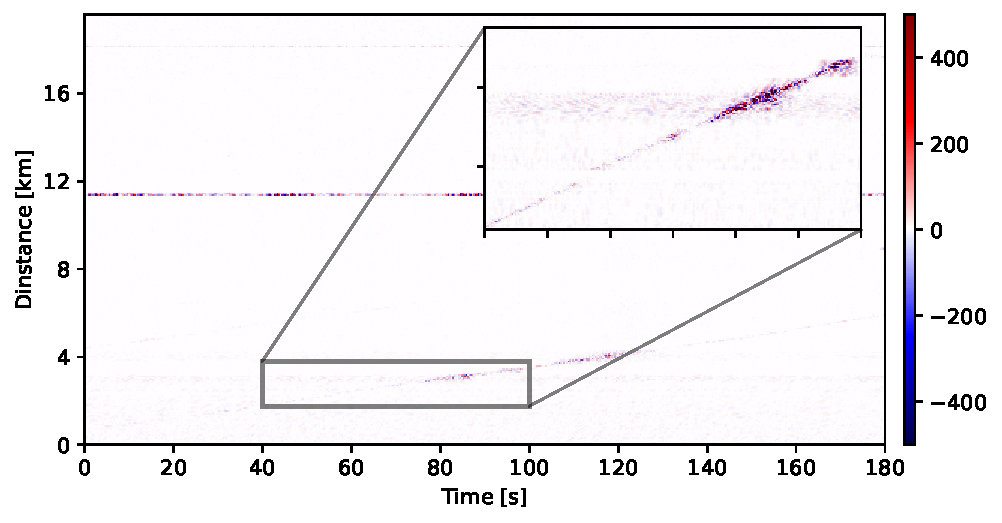
\includegraphics[width=0.8\textwidth]{./out/figure_06_1.pdf}};
        \node (e2) at (5,-5) {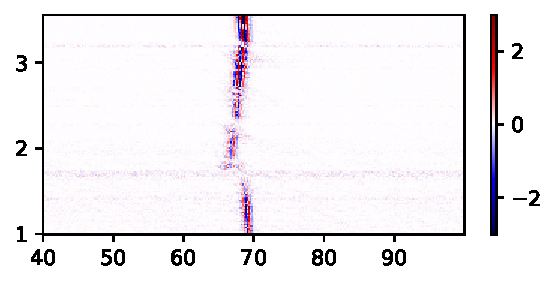
\includegraphics[width=0.4\textwidth]{./out/figure_06_2.pdf}};
        \node (e3) at (-2,-5) {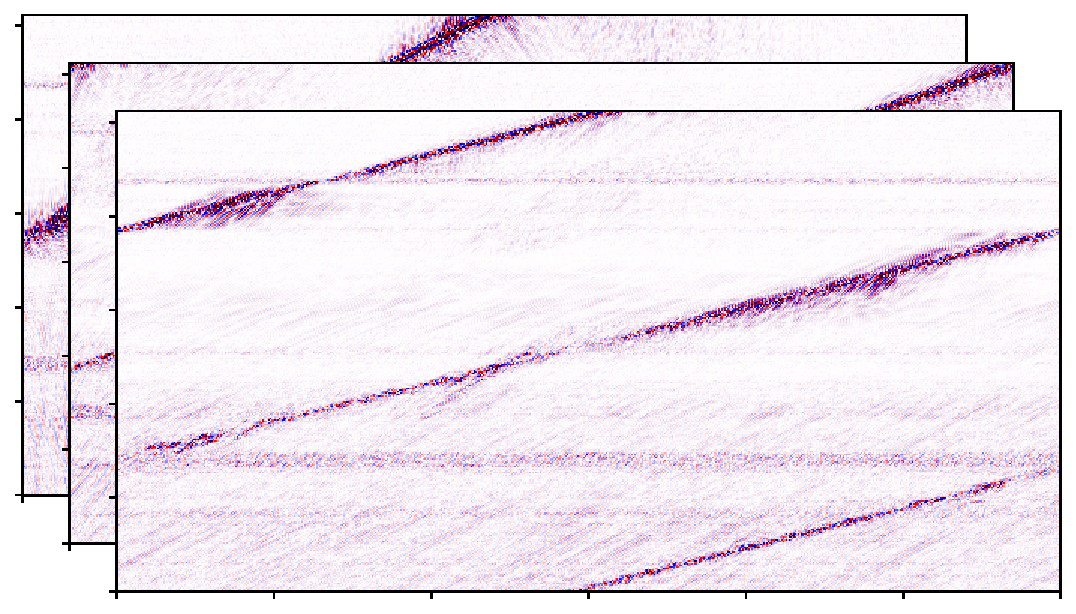
\includegraphics[width=0.4\textwidth]{./out/figure_06_3.pdf}};

        \node (a) at (-5,3) {\Large \textbf{a}};
        \draw [->, thick] ([shift={(0,-1.5)}]e1.north east) -| ([shift={(1.5,0)}]e2.north) node[above=100pt, right] {\Large \textbf{b}}; 
        \draw [->, thick] (e2) -- (e3) node[midway, above] {\Large \textbf{c}}; 
    \end{tikzpicture}
\end{document}